\chapter{Perception}

\section{Perception of lightness \cite{wikipedia_lightness} is not linear}
\begin{figure}[H]
  %\vspace{-2ex}
  \centering
  
\includegraphics[width=0.9\textwidth]{horizontal}
  \caption[Perception of lightness is not linear (1).]{In each row, the \popup{gradient}{The amount of change.} is 1 (0 in each column).}
  \label{fig:HVS_no_linear}
\end{figure}

\begin{figure}[H]
  %\vspace{-2ex}
  \centering
  
\includegraphics[width=0.9\textwidth]{horizontal_vertical}
  \caption[Perception of lightness is not linear (2).]{In each row and column, the \popup{gradient}{The amount of change.} 1.}
  \label{fig:HVS_no_linear}
\end{figure}

\section{Perception of the luminance VS the frequency}
\begin{itemize}
\item The perception of a change of the intensity varies with the spatial frequency.
\begin{figure}[H]
  %\vspace{-2ex}
  \centering
  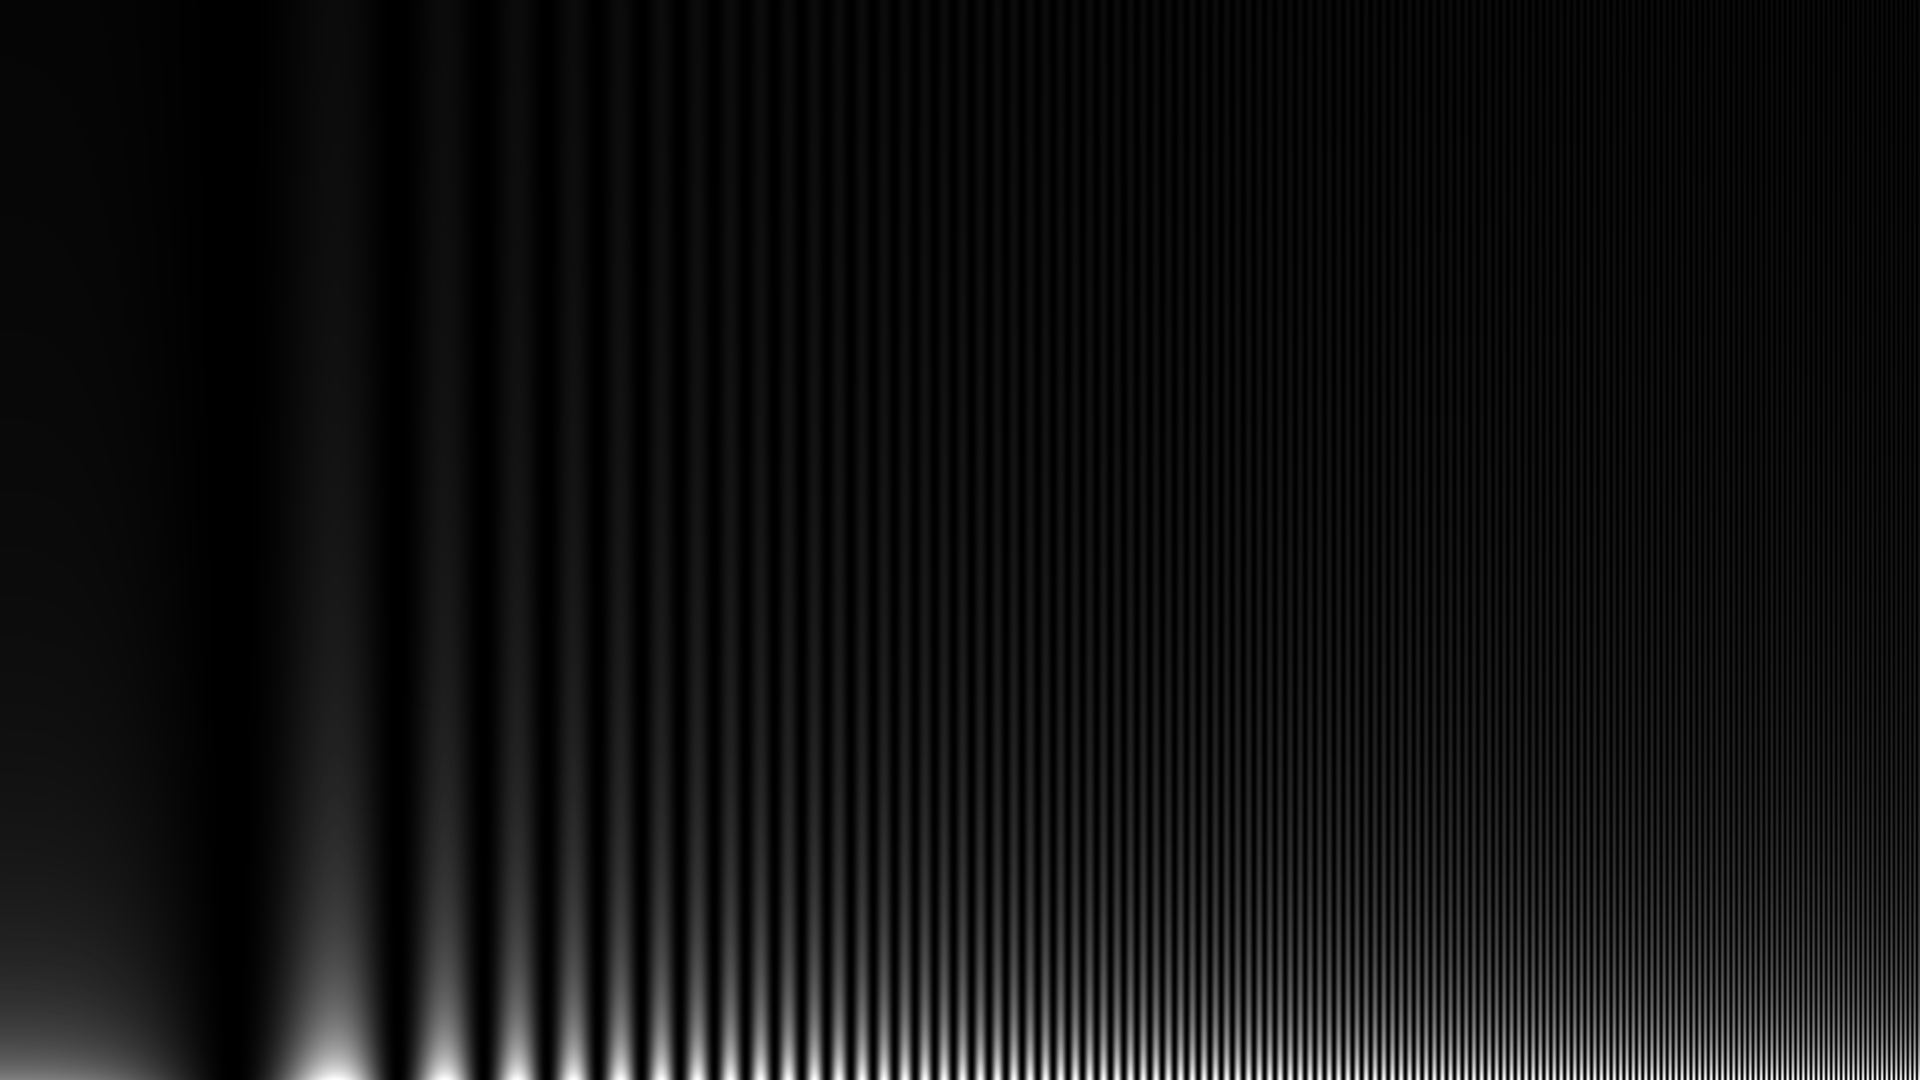
\includegraphics[width=0.65\textwidth]{CSF3}
  \caption{The \gls{CSF}.}
  \label{fig:CSF}
\end{figure}
\end{itemize}

\section{Perception of the \popup{luma}{Luminance.} VS the neighborhood}
\begin{itemize}
\item The perception of the intensity depends the neighbour pixels.
\begin{figure}[H]
  %\vspace{-2ex}
  \centering
  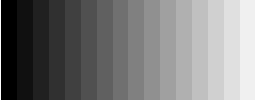
\includegraphics[width=0.8\textwidth]{linear3}
  \caption[Effect of the neighborhood in the perception of the luminance (1).]{Effect of the neighborhood in the perception of the luminance (in each block, all the pixels have the same intensity).}
  \label{fig:luminance_vs_neighbor_1}
\end{figure}
\end{itemize}

\section*{}
\begin{itemize}
\item The perception of the intensity depends the neighbour pixels.
\begin{figure}[H]
  %\vspace{-2ex}
  \centering
  
\includegraphics[width=1.0\textwidth]{contraste_simultaneo}
  \caption[Effect of the neighborhood in the perception of the luminance (2).]{Effect of the neighborhood in the perception of the luminance (all the internal squares have the same intensity).}
  \label{fig:luminance_vs_neighbor_2}
\end{figure}
\end{itemize}

\section{Perception of the luma VS the visualization time}
\begin{itemize}
\item The perception of the intensity depends the visualization time.
\begin{figure}[H]
  %\vspace{-2ex}
  \centering
  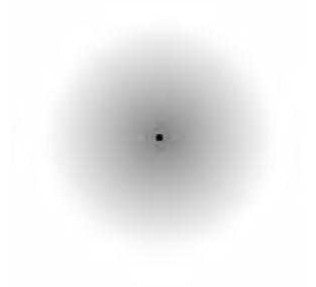
\includegraphics[width=0.4\textwidth]{punto_y_difuminado}
  \caption[Effect of visualization time in the perception of the luminance.]{Effect of the visualization time in the perception of the luminance (look to the central point for a while).}
  \label{fig:luminance_vs_visualization_time}
\end{figure}
\end{itemize}

\section{Noise masking}
\begin{itemize}
\item The perception of the structures depends on the type and intensity of the noise.
\begin{figure}[H]
  %\vspace{-2ex}
  \centering
  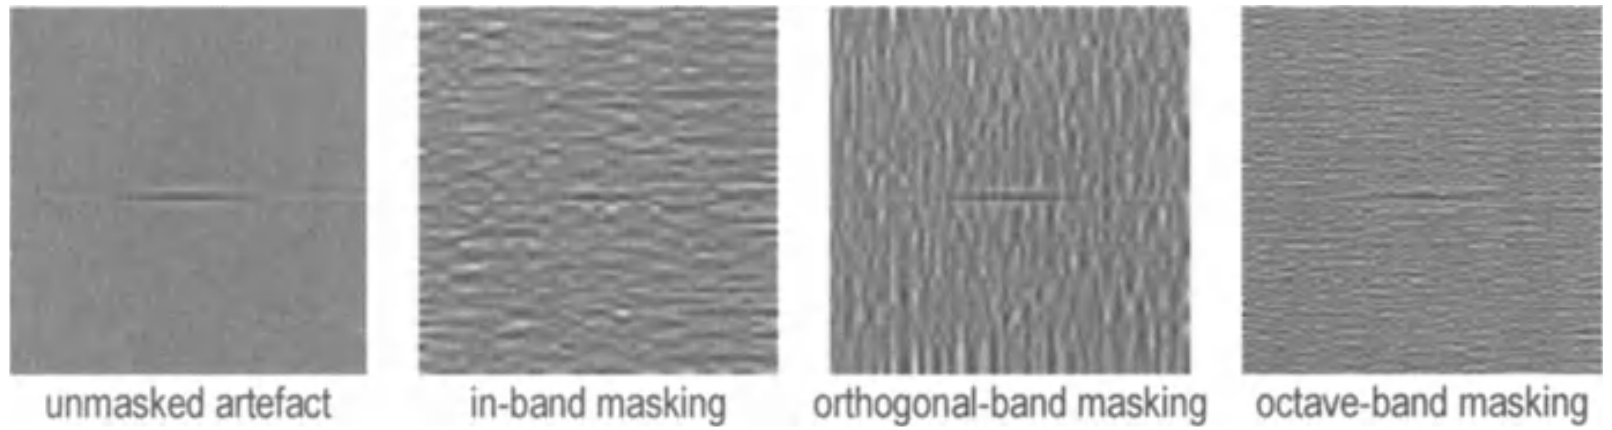
\includegraphics[width=1.0\textwidth]{noise_masking}
  \caption[Noise masking effect.]{Effect of the noise texture in the perception of the luminance (different effects of Gaussian noise in the wavelet domain).}
  \label{fig:noise_masking}
\end{figure}
\end{itemize}
